%----------------------------------------------------------------------------
%bb defines the bounding box for the pdf
%viewport defines the area of the pdf used
%in sidewaysfigure the last entry in bb moves the caption toward/away the pic
%in sidewaysfigure the second entry in bb moves the pic toward/away the caption
%----------------------------------------------------------------------------
\begin{figure}
\scalebox{0.8}[0.8]{
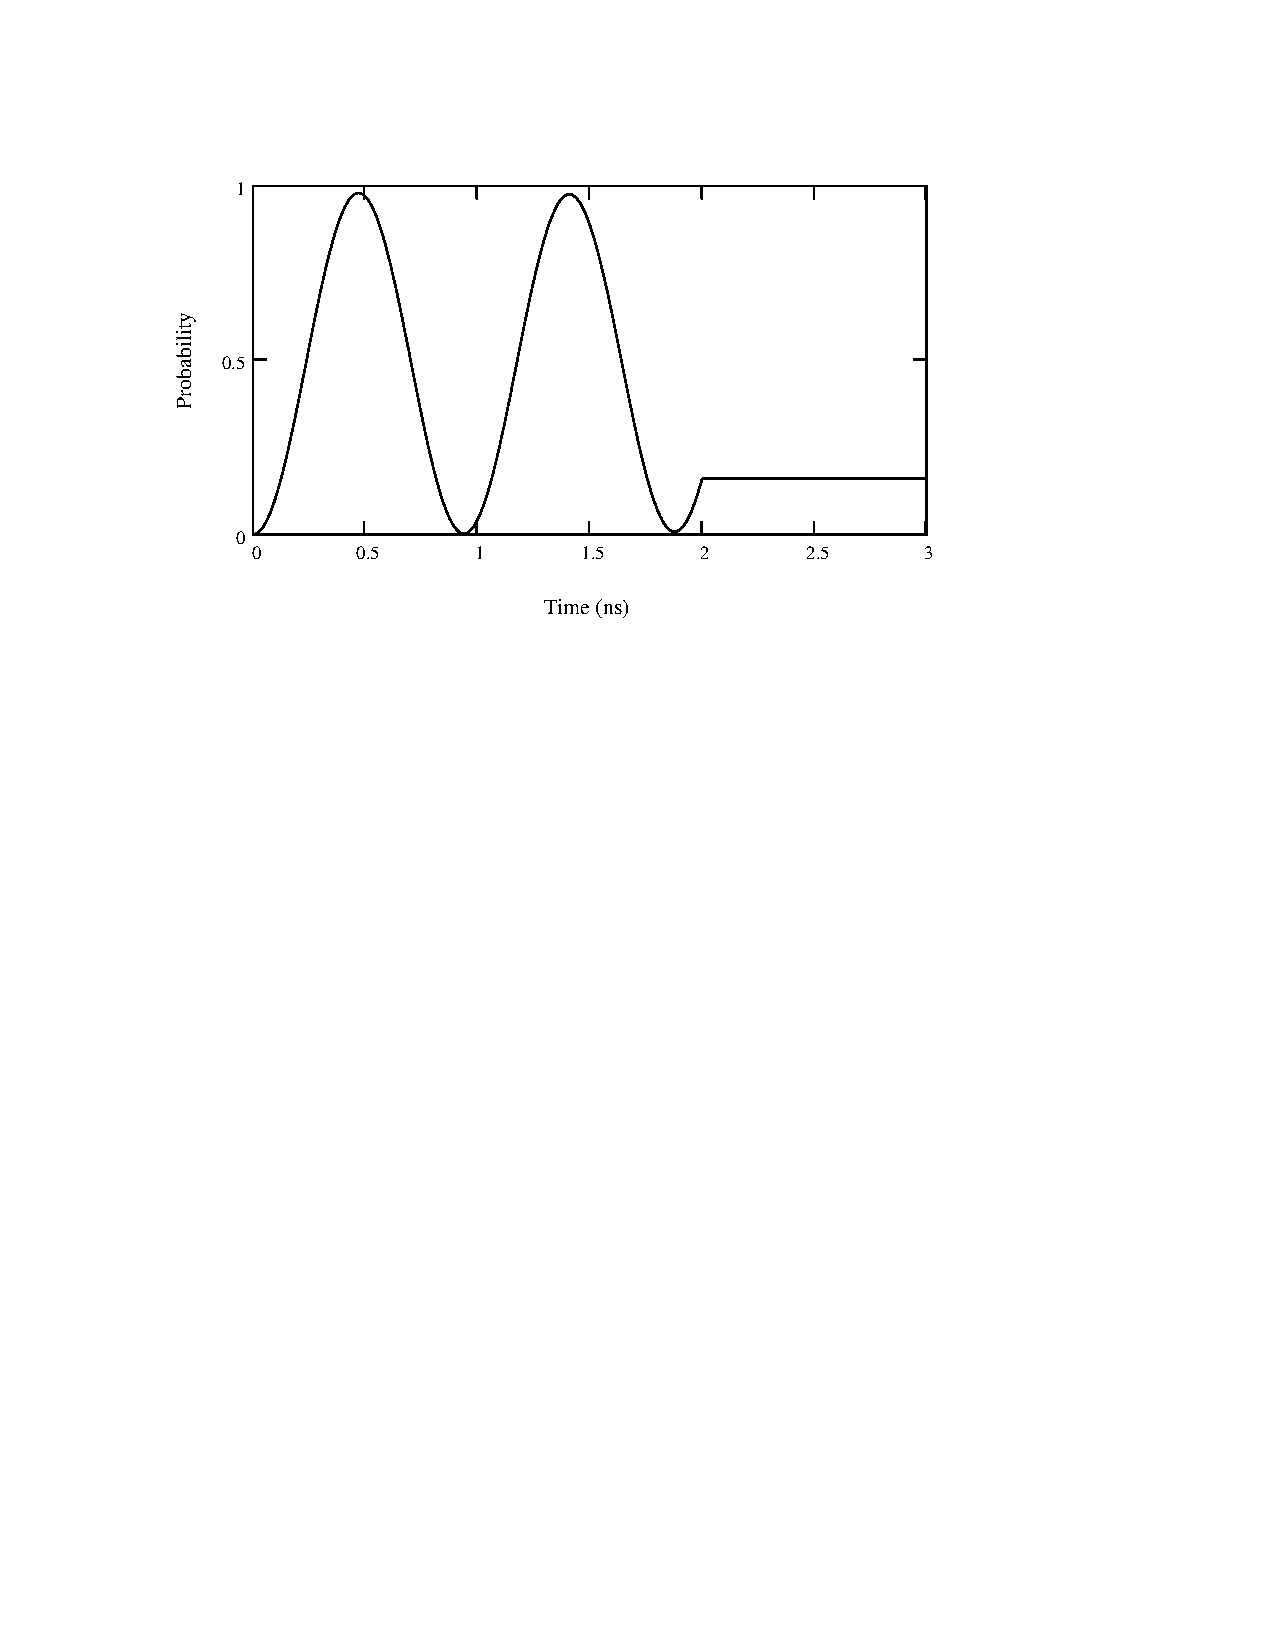
\includegraphics[bb=10 490 550 690]
{thermal_2/thermal_2.pdf}
}
\caption[Simulated thermal (Doppler and geometric) effects on observed fluorescence -- 2 ns pulse]{Simulated thermal (Doppler and geometric) effects on observed fluorescence -- 2 ns pulse. For this simulation a top hat pulse (temporal and spatial) with duration 2 ns, fluence of 1000 J/m$^2$, and beam diameter 1 mm (about 1 mJ per pulse), excites a thermal molecular iodine gas, with dipole matrix element $3.6\cross10^{-32}$ Cm (including FCF), at T = 293K.  The axial dimension of the sensitive region is set to 300 $\mu$m; this is set to the slit width, which is selected such that the J-splitting in iodine fluorescence can still be resolved. The transverse dimension of the sensitive region is set to 0.5 cm (slit mask).}
\label{thermal_2}
\end{figure}
%----------------------------------------------------------------------------
